\documentclass{../UTNetLab}

\title{SDN and Nothing Else}

\begin{document}
\part{SDN Introduction}
    \section{Exercise One}
    Remember one of the previous labs\footnote{Lab 4: Routing} where you are using host rather than router to emulate some routing functionality. In this experiment we want to implement same functionality with SDN switches. To warm up our hands we will start by simple scenario:

    \begin{itemize}
        \item Open \path{switch.py} and read it's codes carefully.
        \item Run this code with \lstbash{sudo python switch.py}
        \item Ping \textit{h2} from the \textit{h1}.
        \item Capture OpenFlow hello packet on the \textit{lo} interface. (Filter \lstbash{wireshark} output with \lstbash{of} filter)
    \end{itemize}

    \begin{report}
        \item Explain line 21 to 26 of \path{switch.py}.
        \item Read \url{http://flowgrammable.org/sdn/openflow/state-machine/} and explain switch handshake with controller. What is \texttt{xid} of your packets. Justify your answer with captured packets. \textbf{Don't copy and paste text from reference in your lab report}.
    \end{report}

    \section{Exercise Two}
    Use what you learned in previous exercise and create \autoref{fig:linearRouters} topology. Configure switches in this topology where ??? we can ping each host from each host. Show your final result to instructors.

    \begin{figure}[H]
        \centering
        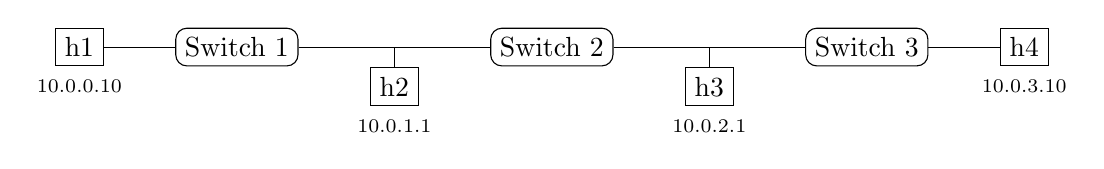
\begin{tikzpicture}
            \draw (0*2,0) node[draw,fill=white] (h1) {h1} +(0,-0.5) node {\scriptsize 10.0.0.10};
            \draw (2*2,-0.5) node[draw,fill=white] (h2) {h2} +(0,-0.5) node {\scriptsize 10.0.1.1};
            \draw (4*2,-0.5) node[draw,fill=white] (h3) {h3} +(0,-0.5) node {\scriptsize 10.0.2.1};
            \draw (6*2,0) node[draw,fill=white] (h4) {h4} +(0,-0.5) node {\scriptsize 10.0.3.10};
            \draw (1*2,0) node[draw,fill=white,rounded corners] (s1) {Switch 1};
            \draw (3*2,0) node[draw,fill=white,rounded corners] (s2) {Switch 2};
            \draw (5*2,0) node[draw,fill=white,rounded corners] (s3) {Switch 3};
            \draw (h1) -- (s1) -- (s2) -- (s3) -- (h4);
            \draw (s1) -| (h2);
            \draw (s2) -| (h3);
        \end{tikzpicture}
        \caption{Mininet topology}
        \label{fig:linearRouters}
    \end{figure}


\part{Exercises with Multitables Flows}
    \section{Exercise Three}
    In this section we are loading switch flows from another files and examining it's functionality.

    \begin{itemize}
        \item Execute \lstbash{sudo python topo.py} 
        \item Execute \lstbash{sh ovs-ofctl add-flows s1 tables.txt} on mininet console.
        \item Ping each host from other hosts.
        \item Capture ICMP packets on each host and observe network behavior.
        \item Modify \path{tables.txt} to drop packets between \textit{h1} and the \textit{h2}.
    \end{itemize}

    \begin{figure}[H]
        \centering
        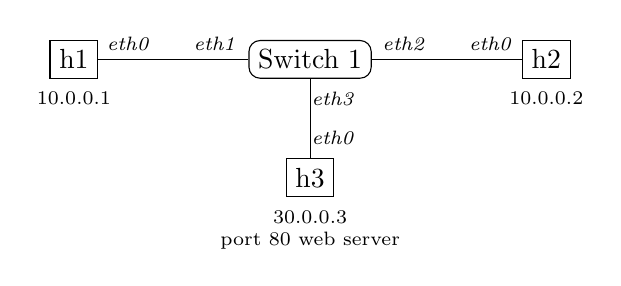
\begin{tikzpicture}
            \draw (0*3,0) node[draw,fill=white] (h1) {h1} ++(0,-0.5) node {\scriptsize 10.0.0.1};
            \draw (1*3,-0.5*3) node[draw,fill=white] (h3) {h3} ++(0,-0.5) node {\scriptsize 30.0.0.3} ++(0,-0.3) node {\scriptsize port 80 web server};
            \draw (2*3,0) node[draw,fill=white] (h2) {h2} ++(0,-0.5) node {\scriptsize 10.0.0.2};
            \draw (1*3,0) node[draw,fill=white,rounded corners] (s1) {Switch 1};
            \draw (s1) -- (h1) +(0.7,0.2) node {\scriptsize\textit{eth0}};
            \draw (s1) +(-0.6*2,0.2) node {\scriptsize\textit{eth1}};
            \draw (s1) -- (h2) +(-0.7,0.2) node {\scriptsize\textit{eth0}};
            \draw (s1) +(0.6*2,0.2) node {\scriptsize\textit{eth2}};
            \draw (s1) -- (h3) +(0.3,0.5) node {\scriptsize\textit{eth0}};
            \draw (s1) +(0.3,-0.5) node {\scriptsize\textit{eth3}};
        \end{tikzpicture}
        \caption{Multitable scenario}
        \label{fig:MultitableScenario}
    \end{figure}


    \begin{report}
        \item Can you explain switch behavior? Justify your answer with \lstbash{wireshark} output and \path{tables.txt} file.
    \end{report}
\end{document}
